
\chapter{Anomalous behavior of spin systems with dipolar interactions}

\section{Introduction}
 We study the properties of spin systems realized by cold polar molecules interacting via dipole-dipole interactions in two-dimensions.
 Using a spin wave theory, that allows for the full treatment of the characteristic long-distance tail of the dipolar interaction, we find several
 anomalous features in the ground state correlations and the spin wave excitation spectrum, which are absent in their counterparts with short range interaction.  The most striking consequence is
 the existence of true long-range order at finite temperature for a two-dimensional phase with a broken $U(1)$ symmetry.





The foundation for understanding the behavior and properties of quantum matter
is based on models with short range interactions.  Experimental progress
in cooling polar molecules \cite{ni08} and atomic gases with large  magnetic dipole moments \cite{griesmaier05}
has  however increased the interest in systems with strong dipole-dipole interactions. While many
properties of quantum systems with dipole-dipole interactions derive from our understanding
of systems with short range interactions,  the dipole-dipole interaction can give rise to phenomena
not present in their short range counterparts. Prominent examples are the description of dipolar
Bose-Einstein condensates, where the contribution of the dipolar interaction can not be included
in the $s$-wave scattering length \cite{lahaye09}, and the absence of  a first order phase transition with a jump in the density \cite{spivak04}.
In this letter, we demonstrate anomalous  behavior  in two-dimensional spin systems with dipolar interactions
realized by polar molecules in optical lattices.

A remarkable property of cold polar molecules confined into two-dimensions  is the potential formation
of  a crystalline phase for strong dipole-dipole interactions \cite{buechler07,astrakharchik07}.  In contrast to a Wigner crystal with Coulomb
interactions \cite{bonsall59}, the crystalline phase exhibits the conventional behavior expected for a crystal realized with a
short range repulsion and the characteristic $1/r^3$ behavior of the dipole interaction can be truncated
at distances involving several inter-particle separations. Several strongly correlated phases have been predicted, which
behave in analogy to systems with  interactions extending over a finite range, such as a Haldane phase \cite{torre06}, supersolids  \cite{pollet10,capogrosso10}, pair supersolids in
bilayer systems \cite{trefzger09}, valence bond solids \cite{bonnes10},
as well as $p$-wave superfluidity \cite{cooper09}, and self-assembled structures in multi-layer setups \cite{wang06}.
%
On the other hand, it has  recently been demonstrated that polar molecules in optical
lattices are also suitable for emulating quantum phases of two-dimensional spin models  \cite{micheli06,gorshkov11,gorshkov11-2}.

Here, we demonstrate that such spin models with dipole-dipole interactions exhibit several anomalous features,
which are not present in their short range counterparts.  The analysis is based on analytical spin wave theory, which
allows for the full treatment of the $1/r^3$ tail of the dipole-dipole interactions. We find that the excitation spectrum
exhibits anomalous behavior at low momenta, which gives rise to unconventional dynamic properties of the spin wave excitations.
Remarkably, we derive from this anomalous behavior the existence of a long-range ordered ferromagnetic phase at finite temperatures;
this finding is consistent with the well-known Mermin-Wagner theorem as the  latter does not exclude order
for interactions with a $1/r^\alpha$ tail, where $\alpha \le 4$ \cite{mermin66,bruno01,sousa05}. Finally, we show that the dipole-dipole interaction gives rise to
algebraic correlations even in gapped ground states, in agreement with recent predictions   \cite{deng05,schuch06}.





\begin{figure}[ht]
 % 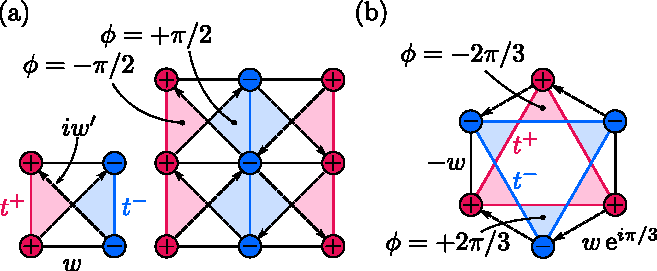
\includegraphics[width= 1\columnwidth]{fig1.eps}
  \caption{(a) Mean-field phase diagram for the XXZ model  with dipolar interactions, where $\tan \theta$ is the ratio between the XY and the Ising spin couplings. (b) Ground state energy per particle:
  the dashed lines show the mean-field predictions,
  while the solid lines include the contributions from the spin waves. At the critical
  values $\theta_{c}$ and $\tilde{\theta}_{c}$,  the ground state energy exhibits the jump $\Delta e_{c}\approx 0.14J$  and $\Delta \tilde{e}_{c}\approx 0.06J$,
  indicating the potential formation of an intermediate phase. }\label{fig1}
\end{figure}





We focus on a setup of polar molecules confined into two-dimensions in a square lattice,
with each lattice site filled by one polar molecule.  A static electric field applied along
the z-direction splits the rotation levels, and allows us to define a spin 1/2 system by selecting
two states in the rotational manifold. Then, the Hamiltonian reduces to a XXZ model with dipole-dipole interaction
between the spins \cite{gorshkov11}
%
\begin{equation}
  H = \frac{ J a^3}{ \hbar^2}\sum_{i \neq j} \frac{\cos \theta \:
S^{z}_{i}S^{z}_{j}+ \sin \theta
\left( S^{x}_{i} S^{x}_{j} + S^{y}_{i} S^{y}_{j}\right) }{|{\bf R}_{i} - {\bf R}_{j}|^3}.
\end{equation}
%
Here, the first term accounts for the static dipole-dipole
interaction between the different rotational levels with strength $J \cos \theta$ , while the last term
describes the virtual exchange of a microwave photon between the two polar molecules with
strength $J \sin \theta$, and  $a$ denotes the lattice spacing.
The dependence of the couplings $J$ and $\theta$ on the microscopic
parameters is discussed in Ref.~\cite{muller10,gorshkov11,gorshkov11-2} and the one-dimensional version of this model has recently been studied in Ref.~\cite{hauke10}.

Before analyzing this spin model on the square lattice, we present a
summary of the phase diagram
for its counterpart with nearest neighbor interactions only.
Then, the phase diagram is highly symmetric and
exhibits four different phases: (i) an Ising
anti-ferromagnetic phase (I-AF) for $-\pi/4 < \theta < \pi/4$ with an
excitation gap, (ii) an XY anti-ferromagnetic phase (XY-AF) for $\pi/4 < \theta
< 3\pi/4$ with a linear excitation spectrum, (iii) an Ising ferromagnetic phase
(I-F) for $3 \pi/4 < \theta < 5\pi/4$ with an excitation gap, and finally (iv) a
XY ferromagnetic phase (XY-F) for $5 \pi/4 < \theta < 7\pi/4$  with a linear
excitation spectrum.


Next, we analyze the modifications of the phase diagram due to dipole-dipole
interactions between the spins within mean-field theory. The
main influence is the reduction of the stability for the antiferromagnetic
phases, as the next-nearest neighbor interaction introduces a  weak frustration
to the system. The ground state energy per lattice site within mean-field
reduces to $  e_{\mbox{\tiny I-AF}} = J \cos \theta \: \epsilon_{\bf K}/4$ and $e_{\mbox{\tiny XY-AF}} = J \sin \theta \: \epsilon_{\bf K}/4$
for the anti-ferromagnetic phases. The summation over the dipole interaction
reduces to a dimensionless parameter $\epsilon_{\bf K} \approx -2.646$, which is related to
the dipolar dispersion
%
\begin{equation}
 \epsilon_{\bf q} = \sum_{j \neq 0} e^{i {\bf R}_{j} {\bf q}}\frac{a^3}{|{\bf R}_{j}|^3}
   \label{dipoledispersion}
\end{equation}
%
at the corner of the Brillouin zone ${\bf K} = (\pi/a, \pi /a)$.
In turn, the ferromagnetic phases are enhanced with a mean-field energy
$e_{\mbox{\tiny I-F}} =  J \cos \theta \: \epsilon_0/4 $  and $ e_{\mbox{\tiny XY-F}} =  J \sin \theta \: \epsilon_0/4$
with $\epsilon_{0}  \approx 9.033$. The modifications to the
phase diagram are shown in Fig.~\ref{fig1}: first, the Heisenberg points at
$\theta = \pi/4,  5 \pi/4$ are protected by the SU(2) symmetry and still
provide the transition between the Ising and the XY phases. However, the
transitions from the ferromagnetic towards the anti-ferromagnetic phase are
shifted to the values  $\theta_{c}= \arctan(\epsilon_{\bf K}/\epsilon_{0})
\approx -0.1 \pi$ and $\tilde{\theta}_c = \pi+ \arctan(\epsilon_{0}/\epsilon_{\bf K})\approx 0.6 \pi$.




\begin{table*}[t]
\begin{tabular}{c c  c}
\toprule
 ground state $\alpha$&  \hspace{30pt}  spin wave excitation spectrum $E^{\alpha}_{\bf q}$   \hspace{30pt} & \hspace{20pt} ground state energy per spin $e_{\alpha}$ \hspace{20pt} \\
 \hline
 \\
I-F& $J \big(\sin \theta  \epsilon_{\bf q} - \cos \theta  \epsilon_{0}\big) $&    $\displaystyle   \frac{3 J \cos \theta \epsilon_{0}}{4}  +\frac{1}{2}  \int \frac{d{\bf q}}{v_0} E_{\alpha}({\bf q})=\frac{J  \cos \theta \epsilon_{0}}{4}$\\
 \\
 XY-F & $    J\sqrt{ \sin\theta \big(\epsilon_{\bf q}-\epsilon_{0}\big)\big( \cos\theta \epsilon_{\bf q}- \sin \theta \epsilon_{0}\big)}$
&$\displaystyle   \frac{3 J \sin \theta \epsilon_{0} }{4}  +\frac{1}{2}  \int \frac{d{\bf q}}{v_0} E^{\alpha}_{\bf q}$\\
\\
 I-AF &  $ J  \sqrt{\big( \sin \theta \epsilon_{{\bf q}+{\bf K}}-\cos \theta \epsilon_{\bf K}\big) \big(\sin \theta \epsilon_{\bf q}- \cos \theta \epsilon_{\bf K }\big)}$
 &$ \displaystyle \frac{3  J \cos \theta \epsilon_{\bf K} }{4}  +\frac{1}{2}  \int \frac{d{\bf q}}{v_0} E^{\alpha}_{\bf q}$\\
 \\
 XY-AF& $  J  \sqrt{\sin \theta \big(  \epsilon_{{\bf q}+{\bf K}}-\epsilon_{\bf K} \big)\big( \cos \theta \epsilon_{\bf q}-\sin \theta \epsilon_{\bf K}\big)}$&
 $\displaystyle \frac{3 J \sin \theta \epsilon_{\bf K} }{4} + \frac{1}{2}  \int \frac{d{\bf q}}{v_0} E^{\alpha}_{\bf q}$\\
\end{tabular}
\caption{ \label{table1} Spin wave excitation spectrum $E_{\bf q}^{\alpha}$ and ground state energy  $e_{\alpha}$.}
\end{table*}



The dipole dispersion $\epsilon_{\bf q}$ in Eq.~(\ref{dipoledispersion})
converges very slowly due to the characteristic power law decay of the dipole-dipole
interaction. It is this slow decay, which will give rise to several peculiar
properties of the system. Therefore, we continue first with a detailed discussion
of this dipolar dispersion.  The precise determination of $\epsilon_{\bf q}$ is
most conveniently performed using an Ewald summation \cite{bonsall59}, which transforms
the summation over the  slowly converging terms with algebraic decay into a summation of exponential factors, i.e.,
%
\begin{eqnarray}
   \epsilon_{\bf q}  & = & - 2 \pi a | {\bf q}|\,{\rm erfc}(a |{\bf q}|/2\sqrt{\pi})   + 4 \pi \left( e^{- \frac{a^2 |{\bf q}|^2}{4 \pi}} - \frac{1}{3}\right)      \label{Ewaldsummation}
\\
   & & \hspace{-20pt}+     2 \pi \sum_{i\neq 0} \int_{1}^{\infty} \! \frac{d \lambda}{ \lambda^{3/2}} \left[ e^{- \pi  \lambda \left(\frac{ {\bf R}_{i}}{a} + \frac{a {\bf q}}{2 \pi}\right)^2} +\lambda^{2}  e^{- \frac{\pi \lambda |{\bf R}_{i}|^2}{a^2}+ i {\bf R}_{i}{\bf q}}\right] \nonumber
   \end{eqnarray}
%
with ${\rm erfc}(x)$ the complementary error function. The important feature of the dipole
dispersion is captured by the first term in Eq.~(\ref{Ewaldsummation}), which
gives rise to a linear and non-analytic behavior $\epsilon_{\bf q} \sim
\epsilon_{0} - 2 \pi a |{\bf q}|$ for small values $q \ll 1/a $, while all
remaining terms are analytic. It is this linear part, which will give rise to
several unconventional properties of spin systems in 2D with dipolar
interactions, and is a consequence of the slow decay of the dipole-dipole
interaction. The summation in the last term converges very quickly and
guarantees the periodicity of the dipolar dispersion. The quantitative behavior
is shown in Fig.~\ref{fig2}a, and the numerical efficient determination provides
$\epsilon_{0}\approx 9.033$, and $\epsilon_{\bf K}=(1/\sqrt{2}-1)  \epsilon_{0}
\approx -2.646$



Next, we analyze the excitation spectrum above the mean-field ground states
within a spin wave analysis. The spin wave analysis is well
established \cite{kubo52,auerbachbook}, and its application for a spin system with dipolar
interaction is straightforward. Details of the calculation are presented in
the supplementary material for the anti-ferromagnetic XY model. The results are
summarized in Table~\ref{table1}, and shown in Fig.~\ref{fig2}. In the following, we present a detailed
discussion for each of the four ordered phases.




\begin{figure}[ht]
 % 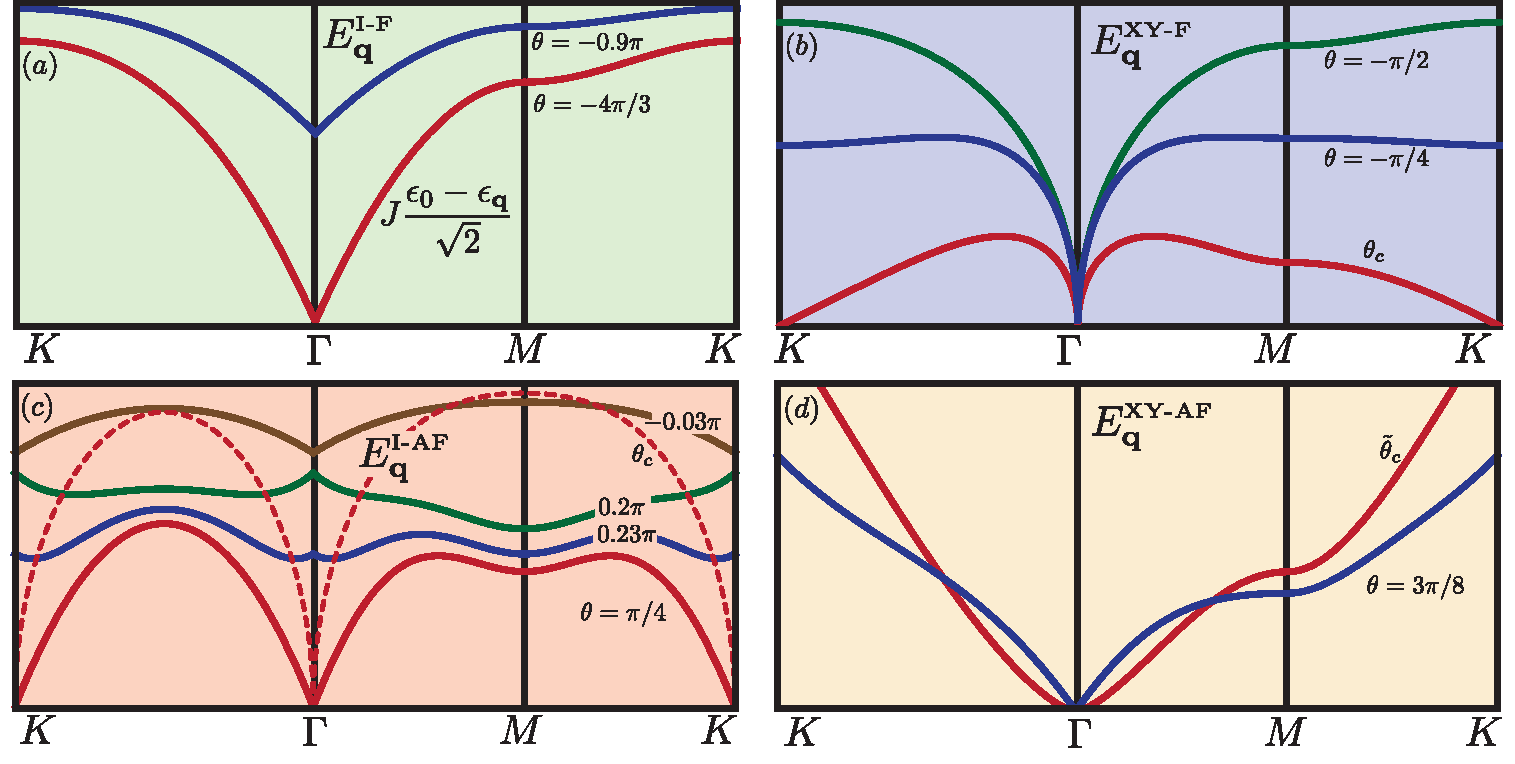
\includegraphics[width= 1\columnwidth]{fig2.eps}
  \caption{Spin wave excitations with $\Gamma=(0,0)$, $M=(0,\pi/2)$, and $K=(\pi/a,\pi/a)$ for different $\theta$ angles. (a) Spectrum of the I-F phase which also shows the behavior of the dipolar dispersion $\epsilon_{\bf q}$ for $\theta=-3\pi/4$, see red line.
(b-d) Spectrum for the XY-F, I-AF and XY-AF phases. Each red line is a critical excitation spectrum indicating an instability.
  }\label{fig2}
\end{figure}




{\it Ising ferromagnetic phase:}
The ferromagnetic mean-field ground state is twofold degenerate with all spins
either point up or down, and is the exact ground state for $\theta =
\pi$, i.e., $|G\rangle = \prod_{i} \left|\downarrow \right\rangle_{i}$. Within the spin wave analysis,
the ground state is not modified and the excitation
spectrum reduces to $E_{{\bf q}}^{\mbox{\tiny I-F}}$, see Table \ref{table1}.
The spin waves exhibit an excitation gap $\Delta$: (i) approaching the
Heisenberg point at  $\theta = -3 \pi /4$, the excitation gap
vanishes, indicating the instability towards the XY ferromagnet, (ii) in
turn, for anti-ferromagnetic XY couplings, the gap is minimal at  ${\bf K}$,
vanishes at the mean-field transition point $\tilde{\theta}_{c}$ and drives an instability towards the formation
of antiferromagnetic ordering.

In contrast to any short range ferromagnetic spin model, the
dispersion relation  $E_{{\bf q}}^{\mbox{\tiny I-F}}$ is not quadratic for small momenta,
but rather exhibits a linear behavior, i.e., $E_{{\bf q}}^{\mbox{\tiny I-F}}   \sim  E_{0}^{\mbox{\tiny I-F}}+ \hbar c |{\bf q}|$ with
velocity $c=  - 2 \pi a J \sin \theta  /\hbar$, which is a consequence of the dipolar interaction in
the system.  This anomalous behavior strongly influences the dynamics
of the spin waves.
The dynamical behavior of a single localized spin excitation is shown in Fig.~\ref{fig3}a for a Gaussian initial state.
In order to probe the linear part in the dispersion relation, the width $\sigma$
of the localization is much larger than the lattice spacing $a$, and therefore, the dynamics is
well described by a continuum description.
Instead of the conventional quantum mechanical spreading, one finds
a ballistic expansion of a cylindrical wave packet with velocity $c$.
In addition, the dipole-dipole interaction also strongly influences the correlation function.
Within conventional perturbation theory, we find algebraic correlations $\langle S_{i}^{x} S_{j}^{x}\rangle \sim 1/|{\bf r}|^3$.
This algebraic decay of correlations even in gapped systems is a peculiar property of
spin models with long-range interactions  \cite{deng05,schuch06}.



\begin{figure}[ht]
 % 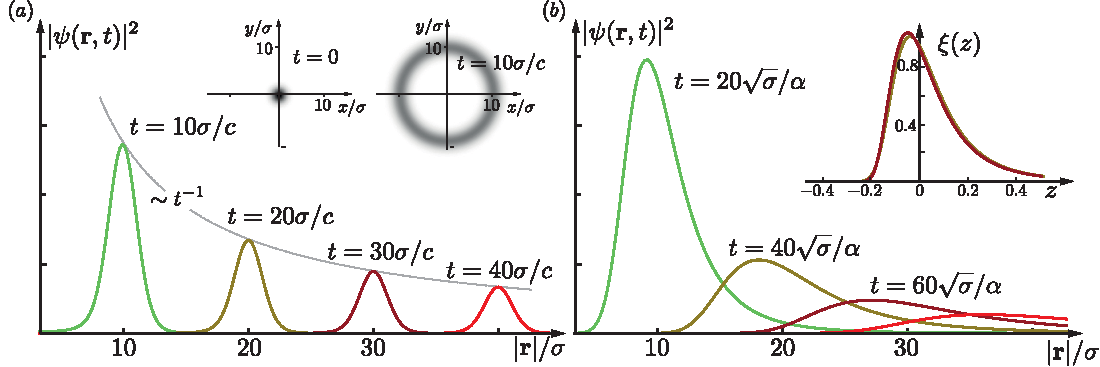
\includegraphics[width= 1\columnwidth]{fig3.eps}
  \caption{ Time evolution for localized spin excitations described by the Gaussian wave packet $\psi_{0}({\bf r}) = e^{- |{\bf r}|^2/2\sigma^2}/\sqrt{\pi \sigma^2}$
  with $\sigma \gg a$ in the continuum description. (a) For a linear dispersion $c|{\bf q}|$ in the I-F phase, the dynamics is described by cylindrical symmetric wave packets (see inset) traveling
  with velocity $c$, instead of the conventional quantum mechanical spreading for massive systems.
  %
  %
  (b)  For an anomalous dispersion with $\alpha \sqrt{|{\bf q}|}$ in the XY-F phase, the behavior at long times $t\gg\sqrt{\sigma} \alpha$ reduces to a
  scaling function $\xi(z)$  via   $|\psi(x,\tau)|^2 = \xi(x/\tau -1/2)/\tau^2$ (see inset) using rescaled
  time $\tau = t \alpha /\sqrt{\sigma}$ and space $x = |{\bf r}|/\sigma$ coordinates. It describes a cylindrical symmetric wave front with velocity
  $\alpha \sqrt{\sigma}$.}\label{fig3}
\end{figure}




 {\it XY-ferromagnetic phase:} Here, the spins are aligned in the xy plane.
 Within the spin wave analysis, we obtain the excitation spectrum
 $ E^{\mbox{\tiny{XY-F}}}_{\bf q}$ and the modified ground state energy
 $e_{\mbox{\tiny{XY-F}}}$.
  In the low momentum regime, the dispersion relation behaves as $ E^{\mbox{\tiny XY-F}}_{\bf q} \sim \sqrt{|{\bf q}|}$,   in contrast to the well
known  linear Goldstone modes for the broken $U(1)$ symmetry.
This anomalous behavior is a peculiar property of the dipolar interaction, and the most crucial consequence
is the existence of long-range order for the continuous broken symmetry at finite temperatures
even in two-dimensions \cite{bruno01}.
This property follows immediately from the above spin wave analysis:
the order parameter reduces to  $m \equiv \Delta m - 1/2=\langle S_{i}^{x}\rangle/\hbar $, where $\Delta m$  accounts for
the suppression of the order parameter by quantum fluctuations. Within spin wave theory, it reduces to ($\Delta m = \langle a^{\dag}_{i} a_{i }\rangle$)
%
\begin{displaymath}
\Delta m\! = \!\!  \int \frac{d{\bf q}}{v_{0}}\left[\frac{\cos \theta \epsilon_{\bf q} +\sin \theta ( \epsilon_{\bf q}-2 \epsilon_{0})}{4 E_{\bf q} } \coth \left(\frac{E_{\bf q}}{2T}\right) - \frac{1}{2}\right] .
\end{displaymath}
%
This expression is finite and small: at $T=0$, the integrand behaves as  $\sim 1/\sqrt{|{\bf q}|}$ and we find a
suppression of the order $\Delta m \approx 0.008$ at $\theta= - \pi/2 $. The smallness of this corrections due to
quantum fluctuations is a good justification for the validity of the spin wave analysis.  On the other hand,
even at finite temperatures, the low momentum behavior of the integrand takes the form $\sim T/|{\bf q}|$,
and provides a finite contribution in contrast to a conventional Goldstone mode, which provides a logarithmic divergence.


The appearance of a long-range order at a finite temperature for a ground state with a broken $U(1)$ symmetry is
a peculiar feature of dipole-dipole interactions, which renders the system more mean-field like.  The system therefore
exhibits a finite temperature transition at a critical temperature $T_{c}$ into a disordered phase; such a behavior is
consistent with the classical XY model with dipolar interactions \cite{bruno01}. The correlation functions determined
within spin wave theory and a high temperature expansion are summarized in Table \ref{table2}.
 Note, that the spin wave analysis neglects the influence of vortices. This is well justified here,
as the dipolar interactions gives rise to a  confining of vortices, i.e., the interaction potential
between a vortex--anti-vortex pair increases linearly with the separation between the vortices.

The spin wave dynamics caused by the anomalous dispersion relation $\sim \sqrt{|{\bf q}|}$ are shown in Fig.~\ref{fig3}b for a Gaussian wave packet of width $\sigma$. Interestingly, the propagation velocity of the wave packets is proportional to $\sqrt{\sigma}$ and thus faster for broad wave packets, in contrast to the usual dispersion dynamics. This is a consequence of the group velocity $v_{\bf q} \sim 1/\sqrt{|{\bf q}|}$ which is large for the small momentum components involved in the broad wave packets.

\begin{table}
\begin{tabular}{c c c c}
\toprule
 correlation function &  \hspace{10pt} $T=0$    \hspace{10pt}&   \hspace{10pt} $0 < T< T_{c}$    \hspace{10pt}&   \hspace{10pt}$T_{c}< T $    \hspace{10pt}\\
 \hline
$ \langle S^{z}_{i} S^{z}_{j}\rangle$  &$ \sim |{\bf r}|^{-5/2}$  & $\sim |{\bf r}|^{-3}$ &  $\sim |{\bf r}|^{-3}$ \\
$ \langle S^{y}_{i} S^{y}_{j}+ S^{x}_{i} S^{x}_{j}\rangle- m^2$  &$ \sim |{\bf r}|^{-3/2}$ &  $\sim |{\bf r}|^{-1}$ &  $\sim |{\bf r}|^{-3}$
\end{tabular}
\caption{ \label{table2} Correlation functions in the XY-F phase predicted by the spin wave analysis and high temperature expansion. }
\end{table}





{\it Ising antiferromagnetic phase}: Next, we focus on the antiferromagnetic phases and start with the I-AF ground state.
Again, the ground state is two-fold degenerate on bipartite lattices.  We choose the ground state with spin up on sublattice $A$
and spin down on sublattice $B$, i.e., $|G\rangle = \prod_{i \in A} \left|\uparrow\right\rangle_{i} \prod_{j\in B} \left|\downarrow\right\rangle_{j}$.
The spin wave analysis is straightforward (see supplement), and we obtain
the spin wave excitation spectrum $ E^{\mbox{\tiny I-AF}}_{\bf q}$ and ground state energy $ e_{\mbox{\tiny I-AF}}$, see Table \ref{table1}.
The system exhibits an excitation gap as expected for a system with a broken $Z_{2}$ symmetry.
However, the dipole interactions give rise to an anomalous behavior at small momenta similar to
the ferromagnetic Ising phase with  $E^{\mbox{\tiny I-AF}}_{\bf q}- E^{\mbox{\tiny I-AF}}_{0} \sim -
\sin \theta |{\bf q}|$.  Consequently, the dynamics of spin waves at low momenta is in analogy to the
Ising-ferromagnet,  see Fig.~\ref{fig3}.  Within spin wave theory, we obtain that the anti-ferromagnetic correlations
%\langle S_{i}^{\beta}S_{j}^{\beta} e^{i {\bf K}( {\bf R}_{i}-{\bf R}_{j})} \rangle$
%$\langle S_{i}^{\beta}S_{j}^{\beta} e^{i {\bf K}{\bf R}_{i j}} \rangle$ with ${\bf R}_{i j} = {\bf R}_{i}- {\bf R}_{j}$
$\langle (-1)^{i-j} S_{i}^{\beta}S_{j}^{\beta} \rangle$
as well as the ferromagnetic correlations  $\langle S_{i}^{\beta}S_{j}^{\beta} \rangle$ decay with the
power law  $\sim1/ |{\bf r}|^{3}$ with $\beta = x,y,z$ determined by the characteristic behavior of the dipole-dipole interaction.
The excitation gap vanishes approaching the mean field critical point $\theta_{c}$ towards XY- ferromagnetic
phase, and also approaching the Heisenberg point at $\theta = \pi/4$. For the latter, the qualitative behavior of the excitation spectrum
changes drastically within a very narrow range of $\theta$, see Fig.~\ref{fig2}c.



{\it XY antiferromagnetic phase}:  Finally, we analyze  the properties of the antiferromagnetic XY phase.
In contrast to the ferromagnetic XY phase, the excitation spectrum  $E^{\mbox{\tiny XY-AF}}_{\bf q}$
exhibits the conventional linear Goldstone mode, see Fig.~\ref{fig2}d. This can be understood, as the
anti-ferromagnetic ordering introduces a cancellation of the dipolar interactions, and provides a behavior in analogy to
its short range counter part: true long-range order exists only at $T=0$, while at finite temperature the system
exhibits quasi long-range order and eventually undergoes a Kosterlitz-Thouless transition for increasing temperature.
Nevertheless, the dipole-dipole interactions give rise to the characteristic algebraic correlations, e.g.,
$\langle (-1)^{i-j}S_{i}^{z}S_{j}^{z} \rangle \sim 1/|{\bf r}|^3$ for the anti-ferromagnetic transverse spin correlation at zero temperature.



Finally, we comment on the transitions between the different phases. The spin wave analysis predicts,
that the excitation spectrum for each phase becomes unstable at the mean-field critical points: For the Heisenberg
points at $\theta = \pi/4, 5\pi/4$, such a behavior is expected due to the enhanced symmetry and one indeed finds,
that at the critical point, the excitation spectrum from the Ising phase coincides with the spectrum from the XY ground state.
Consequently, the spin waves provide the same  contribution to the ground state energy, see Fig.~\ref{fig1}b. In turn, at the instability points
$\theta_{c}$ and $\tilde{\theta}_{c}$, the excitation spectrum from the anti-ferromagnetic phase is different from the spectrum for the ferromagnetic $F$ phase.
Consequently, the ground state energy within the spin wave analysis exhibits a jump, see Fig.~\ref{fig1}a. Such a behavior is an indication
for the appearance of an intermediate phase. However,  this question can not be conclusively answered within the presented analysis due to  the limited validity of spin wave theory close to the transition points. However, the appearance of a first order phase transition can be excluded by arguments similar as in
Ref.~\cite{spivak04}.
